% Created by tikzDevice version 0.10.1 on 2019-05-06 17:11:10
% !TEX encoding = UTF-8 Unicode
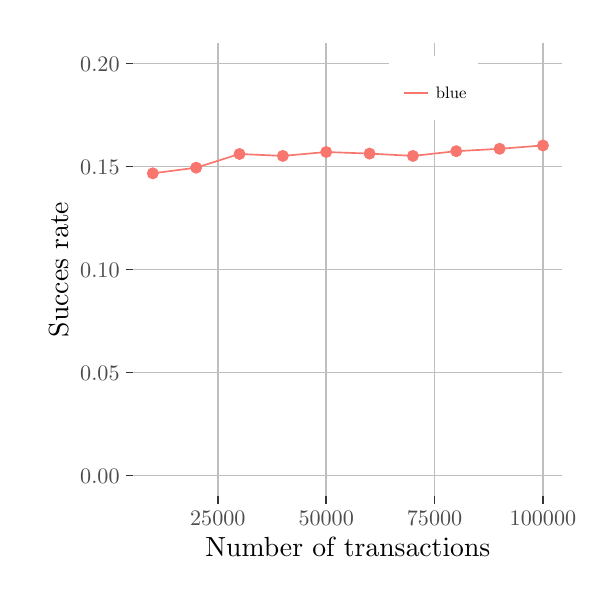
\begin{tikzpicture}[x=1pt,y=1pt]
\definecolor{fillColor}{RGB}{255,255,255}
\path[use as bounding box,fill=fillColor,fill opacity=0.00] (0,0) rectangle (198.74,198.74);
\begin{scope}
\path[clip] (  0.00,  0.00) rectangle (198.74,198.74);
\definecolor{drawColor}{RGB}{255,255,255}
\definecolor{fillColor}{RGB}{255,255,255}

\path[draw=drawColor,line width= 0.6pt,line join=round,line cap=round,fill=fillColor] (  0.00,  0.00) rectangle (198.74,198.74);
\end{scope}
\begin{scope}
\path[clip] ( 38.16, 29.45) rectangle (193.24,193.24);
\definecolor{drawColor}{RGB}{255,255,255}

\path[draw=drawColor,line width= 0.3pt,line join=round] ( 38.16, 55.51) --
	(193.24, 55.51);

\path[draw=drawColor,line width= 0.3pt,line join=round] ( 38.16, 92.73) --
	(193.24, 92.73);

\path[draw=drawColor,line width= 0.3pt,line join=round] ( 38.16,129.96) --
	(193.24,129.96);

\path[draw=drawColor,line width= 0.3pt,line join=round] ( 38.16,167.18) --
	(193.24,167.18);

\path[draw=drawColor,line width= 0.3pt,line join=round] ( 49.12, 29.45) --
	( 49.12,193.24);

\path[draw=drawColor,line width= 0.3pt,line join=round] ( 88.28, 29.45) --
	( 88.28,193.24);

\path[draw=drawColor,line width= 0.3pt,line join=round] (127.45, 29.45) --
	(127.45,193.24);

\path[draw=drawColor,line width= 0.3pt,line join=round] (166.61, 29.45) --
	(166.61,193.24);
\definecolor{drawColor}{RGB}{190,190,190}

\path[draw=drawColor,line width= 0.6pt,line join=round] ( 38.16, 36.89) --
	(193.24, 36.89);

\path[draw=drawColor,line width= 0.6pt,line join=round] ( 38.16, 74.12) --
	(193.24, 74.12);

\path[draw=drawColor,line width= 0.6pt,line join=round] ( 38.16,111.34) --
	(193.24,111.34);

\path[draw=drawColor,line width= 0.6pt,line join=round] ( 38.16,148.57) --
	(193.24,148.57);

\path[draw=drawColor,line width= 0.6pt,line join=round] ( 38.16,185.80) --
	(193.24,185.80);

\path[draw=drawColor,line width= 0.6pt,line join=round] ( 68.70, 29.45) --
	( 68.70,193.24);

\path[draw=drawColor,line width= 0.6pt,line join=round] (107.87, 29.45) --
	(107.87,193.24);

\path[draw=drawColor,line width= 0.6pt,line join=round] (147.03, 29.45) --
	(147.03,193.24);

\path[draw=drawColor,line width= 0.6pt,line join=round] (186.19, 29.45) --
	(186.19,193.24);
\definecolor{drawColor}{RGB}{248,118,109}
\definecolor{fillColor}{RGB}{248,118,109}

\path[draw=drawColor,line width= 0.4pt,line join=round,line cap=round,fill=fillColor] ( 45.21,146.11) circle (  1.96);

\path[draw=drawColor,line width= 0.4pt,line join=round,line cap=round,fill=fillColor] ( 60.87,148.14) circle (  1.96);

\path[draw=drawColor,line width= 0.4pt,line join=round,line cap=round,fill=fillColor] ( 76.54,153.10) circle (  1.96);

\path[draw=drawColor,line width= 0.4pt,line join=round,line cap=round,fill=fillColor] ( 92.20,152.40) circle (  1.96);

\path[draw=drawColor,line width= 0.4pt,line join=round,line cap=round,fill=fillColor] (107.87,153.81) circle (  1.96);

\path[draw=drawColor,line width= 0.4pt,line join=round,line cap=round,fill=fillColor] (123.53,153.24) circle (  1.96);

\path[draw=drawColor,line width= 0.4pt,line join=round,line cap=round,fill=fillColor] (139.20,152.40) circle (  1.96);

\path[draw=drawColor,line width= 0.4pt,line join=round,line cap=round,fill=fillColor] (154.86,154.11) circle (  1.96);

\path[draw=drawColor,line width= 0.4pt,line join=round,line cap=round,fill=fillColor] (170.53,154.97) circle (  1.96);

\path[draw=drawColor,line width= 0.4pt,line join=round,line cap=round,fill=fillColor] (186.19,156.18) circle (  1.96);

\path[draw=drawColor,line width= 0.6pt,line join=round] ( 45.21,146.11) --
	( 60.87,148.14) --
	( 76.54,153.10) --
	( 92.20,152.40) --
	(107.87,153.81) --
	(123.53,153.24) --
	(139.20,152.40) --
	(154.86,154.11) --
	(170.53,154.97) --
	(186.19,156.18);
\end{scope}
\begin{scope}
\path[clip] (  0.00,  0.00) rectangle (198.74,198.74);
\definecolor{drawColor}{gray}{0.30}

\node[text=drawColor,anchor=base east,inner sep=0pt, outer sep=0pt, scale=  0.80] at ( 33.21, 34.14) {0.00};

\node[text=drawColor,anchor=base east,inner sep=0pt, outer sep=0pt, scale=  0.80] at ( 33.21, 71.36) {0.05};

\node[text=drawColor,anchor=base east,inner sep=0pt, outer sep=0pt, scale=  0.80] at ( 33.21,108.59) {0.10};

\node[text=drawColor,anchor=base east,inner sep=0pt, outer sep=0pt, scale=  0.80] at ( 33.21,145.82) {0.15};

\node[text=drawColor,anchor=base east,inner sep=0pt, outer sep=0pt, scale=  0.80] at ( 33.21,183.04) {0.20};
\end{scope}
\begin{scope}
\path[clip] (  0.00,  0.00) rectangle (198.74,198.74);
\definecolor{drawColor}{gray}{0.20}

\path[draw=drawColor,line width= 0.6pt,line join=round] ( 35.41, 36.89) --
	( 38.16, 36.89);

\path[draw=drawColor,line width= 0.6pt,line join=round] ( 35.41, 74.12) --
	( 38.16, 74.12);

\path[draw=drawColor,line width= 0.6pt,line join=round] ( 35.41,111.34) --
	( 38.16,111.34);

\path[draw=drawColor,line width= 0.6pt,line join=round] ( 35.41,148.57) --
	( 38.16,148.57);

\path[draw=drawColor,line width= 0.6pt,line join=round] ( 35.41,185.80) --
	( 38.16,185.80);
\end{scope}
\begin{scope}
\path[clip] (  0.00,  0.00) rectangle (198.74,198.74);
\definecolor{drawColor}{gray}{0.20}

\path[draw=drawColor,line width= 0.6pt,line join=round] ( 68.70, 26.70) --
	( 68.70, 29.45);

\path[draw=drawColor,line width= 0.6pt,line join=round] (107.87, 26.70) --
	(107.87, 29.45);

\path[draw=drawColor,line width= 0.6pt,line join=round] (147.03, 26.70) --
	(147.03, 29.45);

\path[draw=drawColor,line width= 0.6pt,line join=round] (186.19, 26.70) --
	(186.19, 29.45);
\end{scope}
\begin{scope}
\path[clip] (  0.00,  0.00) rectangle (198.74,198.74);
\definecolor{drawColor}{gray}{0.30}

\node[text=drawColor,anchor=base,inner sep=0pt, outer sep=0pt, scale=  0.80] at ( 68.70, 18.99) {25000};

\node[text=drawColor,anchor=base,inner sep=0pt, outer sep=0pt, scale=  0.80] at (107.87, 18.99) {50000};

\node[text=drawColor,anchor=base,inner sep=0pt, outer sep=0pt, scale=  0.80] at (147.03, 18.99) {75000};

\node[text=drawColor,anchor=base,inner sep=0pt, outer sep=0pt, scale=  0.80] at (186.19, 18.99) {100000};
\end{scope}
\begin{scope}
\path[clip] (  0.00,  0.00) rectangle (198.74,198.74);
\definecolor{drawColor}{RGB}{0,0,0}

\node[text=drawColor,anchor=base,inner sep=0pt, outer sep=0pt, scale=  1.00] at (115.70,  7.70) {Number of transactions};
\end{scope}
\begin{scope}
\path[clip] (  0.00,  0.00) rectangle (198.74,198.74);
\definecolor{drawColor}{RGB}{0,0,0}

\node[text=drawColor,rotate= 90.00,anchor=base,inner sep=0pt, outer sep=0pt, scale=  1.00] at ( 14.59,111.34) {Succes rate};
\end{scope}
\begin{scope}
\path[clip] (  0.00,  0.00) rectangle (198.74,198.74);
\definecolor{fillColor}{RGB}{255,255,255}

\path[fill=fillColor] (130.63,165.37) rectangle (162.81,188.36);
\end{scope}
\begin{scope}
\path[clip] (  0.00,  0.00) rectangle (198.74,198.74);
\definecolor{drawColor}{RGB}{248,118,109}

\path[draw=drawColor,line width= 0.6pt,line join=round] (135.98,175.06) -- (144.65,175.06);
\end{scope}
\begin{scope}
\path[clip] (  0.00,  0.00) rectangle (198.74,198.74);
\definecolor{drawColor}{RGB}{0,0,0}

\node[text=drawColor,anchor=base west,inner sep=0pt, outer sep=0pt, scale=  0.60] at (147.54,172.99) {blue};
\end{scope}
\end{tikzpicture}
